\documentclass[a4paper,11pt]{article} % screen setting

\usepackage[a4paper]{geometry}
\geometry{verbose,tmargin=1.5cm,bmargin=1.5cm,lmargin=1.5cm,rmargin=1.5cm}

\setlength{\parskip}{\smallskipamount}
\setlength{\parindent}{0pt}

%\usepackage{fontspec}
\usepackage[libertine]{newtxmath}
\usepackage[no-math]{fontspec}
\setmainfont{Linux Libertine O}
\setmonofont{DejaVu Sans Mono}

\usepackage{hyperref}
\usepackage{url}
\usepackage{xcolor}

% DARKMODE
%\pagecolor[rgb]{0,0,0} %black
%\color[rgb]{0.8,0.8,0.8} %grey

\usepackage{amsmath}
\usepackage{amssymb}

\usepackage{graphicx}
\usepackage{float}

\usepackage{minted}

\newminted{dart}{breaklines,fontsize=\footnotesize}
\newminted{bash}{breaklines,fontsize=\footnotesize}
\newminted{text}{breaklines,fontsize=\footnotesize}

\newcommand{\txtinline}[1]{\mintinline[breaklines,fontsize=\footnotesize]{text}{#1}}
\newcommand{\dartinline}[1]{\mintinline[breaklines,fontsize=\footnotesize]{python}{#1}}

\newmintedfile[pythonfile]{python}{breaklines,fontsize=\footnotesize}

\definecolor{mintedbg}{rgb}{0.90,0.90,0.90}
\usepackage{mdframed}
\BeforeBeginEnvironment{minted}{
    \begin{mdframed}[backgroundcolor=mintedbg,%
        topline=false,bottomline=false,%
        leftline=false,rightline=false]
}
\AfterEndEnvironment{minted}{\end{mdframed}}


\usepackage{setspace}

\onehalfspacing

\usepackage{appendix}


\newcommand{\highlighteq}[1]{\colorbox{blue!25}{$\displaystyle#1$}}
\newcommand{\highlight}[1]{\colorbox{red!25}{#1}}


\begin{document}


\title{Pemrograman User Interface dengan Flutter:\\
Form}
\author{Fadjar Fathurrahman}
\date{}
\maketitle

\section{Tujuan}

\begin{itemize}
\item mengimplementasikan form dan validasi data sederhana pada aplikasi Flutter
\end{itemize}

\section{Form}
Pada minggu lalu, kita telah mengenal beberapa widget yang dapat digunakan untuk
menerima input dari user. Widget input ini dapat digabungkan ke dalam suatu widget
\txtinline{Form}. Widget \txtinline{Form} biasa digunakan jika kita ingin mendapatkan
input data yang saling terkait. Misalnya kita ingin membuat suatu fitur untuk menambahkan
user baru pada aplikasi. Biasanya kita memerlukan input nama pengguna (nama asli),
username, password, email, tempat dan tanggal lahir, dan sebagainya. Pada kasus tersebut
\txtinline{Form} dapat digunakan untuk membungkus semua widget input yang diperlukan
beserta data yang ada menjadi suatu kesatuan.
Pada Flutter, \txtinline{Form} dapat melakukan hal ini dengan menggunakan suatu
key, yang dapat diinisialisasi menggunakan sintaks berikut:

\begin{dartcode}
GlobalKey<FormState> _key = GlobalKey<FormState>();
\end{dartcode}

Variabel \txtinline{_key} ini kemudian dapat digunakan pada \txtinline{Form}
sebagai berikut:
\begin{dartcode}
Widget build(BuildContext context) {
  return Form(
    key: _key,
    child: ... //
  );
}
\end{dartcode}

Pada dasarnya, setiap input widget dapat dibungkus dalam suatu \txtinline{Form}.
Flutter menyediakan widget \txtinline{FormField} yang dapat membungkus sembarang widget
sehingga dapat digunakan pada suatu \txtinline{Form}. Salah satu keuntungannya adalah
\txtinline{FormField} menyediakan beberapa metode yang berguna dalam memproses input
dari \txtinline{Form}:
\begin{itemize}
\item \txtinline{onSaved}
\item \txtinline{validator}
\end{itemize}

Pada Flutter, ada satu widget yang sering digunakan pada \txtinline{Form} yang sudah
dibungkus dengan \txtinline{FormField}, yaitu \txtinline{TextFormField}. Widget ini
tidak lain adalah \txtinline{TextField} yang sudah dibungkus dengan \txtinline{FormField}
sehingga dapat langsung digunakan pada \txtinline{Form}.

Contoh:
\begin{dartcode}

// Gunakan widget ini sebagai home pada MaterialApp
class ContohFormPage extends StatelessWidget {
  @override
  Widget build(BuildContext context) {
    return Scaffold(
      appBar: AppBar(title: Text('Contoh Form')),
      body: ContohForm(),
    );
  }
}

class ContohForm extends StatefulWidget {
  @override
  ContohFormState createState() {
    return ContohFormState();
  }
}
  
class ContohFormState extends State<ContohForm> {
  
  final _formKey = GlobalKey<FormState>();
  String _nama = '';
  String _nim = ''; 
  
  @override
  Widget build(BuildContext context) {
  
    final _buttonSubmit = Padding(
      padding: const EdgeInsets.symmetric(vertical: 16.0),
      child: ElevatedButton(
        child: Text('Daftar'),
        onPressed: () {
          Scaffold.of(context).showSnackBar(
            SnackBar(
              content: Text('Terimakasih data sedang diproses')
            )
          );
          // Tulis ke terminal
          print('Nama = $_nama');
          print('NIM  = $_nim');
        },
      ),
    );
  
    final _inputNama = TextFormField(
      decoration: InputDecoration(
        labelText: 'Nama',
        hintText: 'Ketik nama Anda di sini',
      ),
      onChanged: ..., // lengkapi
    );
  
    final _inputNim = TextFormField(
      decoration: InputDecoration(
        labelText: 'NIM',
        hintText: 'Ketik nama Anda di sini',
      ),
      onChanged: ..., // lengkapi
    );

    return Form(
      key: _formKey,
      child: Column(
        crossAxisAlignment: CrossAxisAlignment.start,
        children: <Widget>[
          _inputNama,
          _inputNim,
          _buttonSubmit,
        ],
      ),
    );
  }
}
\end{dartcode}

Contoh tampilan:
\begin{figure}[h]
{\centering
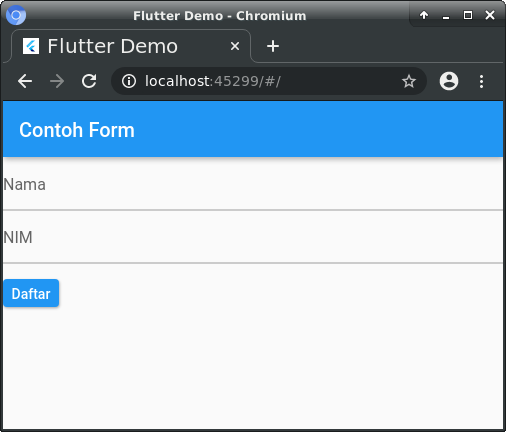
\includegraphics[scale=0.5]{images/simpleform001.png}
\par}
\end{figure}

Silakan lengkapi kode di atas sehingga ketika button Daftar ditekan, program
akan menampilkan nama dan NIM pada terminal atau konsol.


\section{Validasi}

Pada beberapa form, kita seringkali perlu melakukan validasi dari input yang diterima
oleh user. Misalkan kita ingin agar input nama tidak boleh kosong ketika user mengklik
tombol Daftar.
Hal ini dapat dilakukan dengan menggunakan properti \txtinline{validator} pada
\txtinline{_inputNama}:
\begin{dartcode}
final _inputNama = TextFormField(
  decoration: InputDecoration(
    labelText: 'Nama',
    hintText: 'Ketik nama Anda di sini',
  ),
  onChanged: ..., // silakan isi
  validator: (value) {
    if (value.isEmpty) {
      return 'Bagian ini harus diisi';
    }
    return null;
  }
);
\end{dartcode}

Untuk \txtinline{_buttonSubmit}:
\begin{dartcode}
final _buttonSubmit = Padding(
  padding: const EdgeInsets.symmetric(vertical: 16.0),
  child: ElevatedButton(
    child: Text('Daftar'),
    onPressed: () {
      if(_formKey.currentState.validate()) {
        Scaffold.of(context).showSnackBar(
          SnackBar(
            content: Text('Terimakasih data sedang diproses')
          )
        );
        print('nama = $_nama');
        print('NIM  = $_nim');
      }
    },
  ),
);
\end{dartcode}

Tampilan aplikasi:
\begin{figure}[h]
{\centering
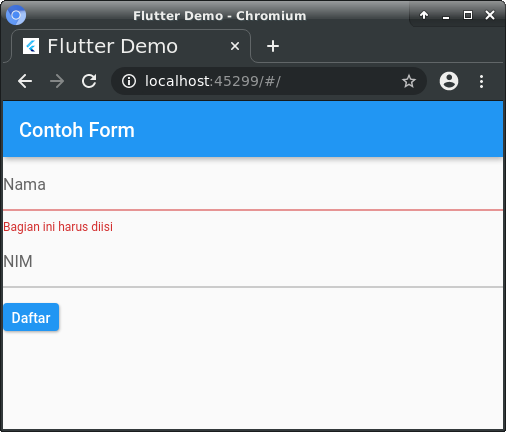
\includegraphics[scale=0.5]{images/simpleform02.png}
\par}
\end{figure}


\section{Tugas}
\begin{itemize}
\item Coba lakukan validasi untuk \txtinline{_inputNim} sehingga input ini harus diisi.
\item Buat suatu data mahasiswa beserta NIM, misalkan untuk 10 mahasiswa. Lakukan
validasi untuk input nama dan NIM yang diberikan sedemikian rupa sehingga hanya nama dan
NIM yang ada pada data yang dapat diterima. Periksa juga sehingga pasangan nama
dan NIM sesuai.
\end{itemize}


\bibliographystyle{unsrt}
\bibliography{BIBLIO}

\end{document}
